\documentclass[tikz,convert={outext=.svg,command=\unexpanded{pdf2svg \infile\space\outfile}},multi=false]{standalone}
\usepackage[utf8]{inputenc}

\begin{document}
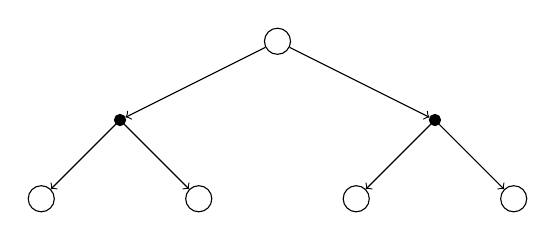
\begin{tikzpicture}
\tikzstyle{state} = [draw, circle, fill=white];
\tikzstyle{action} = [draw, circle, fill=black, inner sep=0.5mm];
\tikzstyle{finalstate} = [draw, fill=gray];
\node[state] (s) {};
\node[action] (a1) at (-2, -1) {};
\node[action] (a2) at (2, -1) {};
\node[state] (s11) at (-3, -2) {};
\node[state] (s12) at (-1, -2) {};
\node[state] (s21) at (1, -2) {};
\node[state] (s22) at (3, -2) {};
\draw[->] (s) -- (a1);
\draw[->] (s) -- (a2);
\draw[->] (a1) -- (s11);
\draw[->] (a1) -- (s12);
\draw[->] (a2) -- (s21);
\draw[->] (a2) -- (s22);
\end{tikzpicture}
\end{document}